\documentclass[11pt]{article}
\usepackage{amsmath, amsfonts, amssymb,amsthm}
\usepackage[includeheadfoot]{geometry} % For page dimensions
\usepackage{fancyhdr}
\usepackage{enumerate} % For custom lists
\usepackage{tikz-cd}
\usepackage{xr}
\externaldocument{427Notes}

\fancyhf{}
\lhead{427 Exercises}
\rhead{Tighe McAsey}
\pagestyle{fancy}

% Page dimensions
\geometry{a4paper, margin=1in}

\theoremstyle{definition}
\newtheorem{pb}{}

% Commands:

\newcommand{\set}[1]{\{#1\}}
\newcommand{\abs}[1]{\lvert#1\rvert}
\newcommand{\norm}[1]{\lvert\lvert#1\rvert\rvert}
\newcommand{\gen}[1]{\left\langle #1 \right\rangle}
\newcommand{\tand}{\text{ and }}
\newcommand{\tor}{\text{ or }}
\newcommand{\falg}{F^{\text{alg}}}
\newcommand{\gal}{\text{Gal}}
\newcommand{\mor}{\text{Mor}}
\newcommand{\floor}[1]{\left\lfloor #1 \right\rfloor}
\newcommand{\im}{\text{Im}}
\title{Exercises}

\begin{document}
\maketitle

\section{Categories and Pre-reqs}

\emph{exercise - }\label{PreEx1} Show the forgetful functor \(F: \text{Vect}_k \to \text{Set}\) is a functor.

\emph{proof - } The identity linear transformation is the identity when regarded as a set mapping, if \(T: U \to V, \varphi: V \to S\) as vector spaces, then \(F(\varphi)\circ F(T)\) is a well defined set mapping, which maps \(U \to S\) as sets.

%%%%%%%%%%%%%%%%%%%%%%%%%%%%%%%%%%%%%%%%%%%%%%%%%%%%%%%%%%%%%%%%%%%%%%%%%%%%%%%%%%%%%%%%%%%%%%%%%%%%%%%%%%%%%%%%%%%%%%%%%%%%%%%%%%%%%%%
%%%%%%%%%%%%%%%%%%%%%%%%%%%%%%%%%%%%%%%%%%%%%%%%%%%%%%%%%%%%%%%%%%%%%%%%%%%%%%%%%%%%%%%%%%%%%%%%%%%%%%%%%%%%%%%%%%%%%%%%%%%%%%%%%%%%%%%

\section{Chain Complexes}\label{CCEx} \ref{CCNotes}

\emph{exercise - }\label{CCEx1} Show that \(\mathbf{h} = (h_i)\), \(h_i: C_i \to C_{i+1}'\), then \(h_{i-1}\circ d_i + d_{i+1}' \circ h_i\) is a chain map.

\emph{proof - } We need to check that \(d_i' \circ f_i = f_{i-1} \circ d_i\), in other words we need to show
\begin{align*}
    d_i' \circ (h_{i-1}\circ d_i + d_{i+1}' \circ h_i) = (h_{i-2}\circ d_{i-1} + d_{i}' \circ h_{i-1})\circ d_i
\end{align*}
Since we are in a module, we can distribute \(d_i'\) on the left hand side, rewriting the condition as
\begin{align*}
    d_i' \circ h_{i-1}\circ d_i + d_i' \circ d_{i+1}' \circ h_i = h_{i-2}\circ d_{i-1}\circ d_i + d_{i}' \circ h_{i-1}\circ d_i
\end{align*}
So it will suffice to show that
\begin{align*}
    d_i' \circ d_{i+1}' \circ h_i = h_{i-2}\circ d_{i-1}\circ d_i
\end{align*}
But this is trivial since "\(d^2 = 0\)"


%%%%%%%%%%%%%%%%%%%%%%%%%%%%%%%%%%%%%%%%%%%%%%%%%%%%%%%%%%%%%%%%%%%%%%%%%%%%%%%%%%%%%%%%%%%%%%%%%%%%%%%%%%%%%%%%%%%%%%%%%%%%%%%%%%%%%%%


\emph{exercise - }\label{CCEx2} A homotopy of chains is an equivalence relation

\emph{proof - } We will prove the following items: reflexivity, symmetry, transitivity
\begin{itemize}
    \item To see that \(f \sim f\), take each to be the zero map, \(h_i = 0, \forall i\). In this case the diagram with maps given by \(\mathbf{h}\) is immediate.
    \item Suppose that \(f \sim g\), then we have some \(\mathbf{h}\), such that \(g_i -f_i = h_{i-1}\circ d_i + d_{i+1}' \circ h_i\) for each \(i\). Since \(h_i\) are morphisms of modules, so are \(-h_i\), so in particular we have \(\mathbf{-h} := (-h_i)_i\), so that 
    \begin{align*}
        f_i - g_i &= -(g_i - f_i) = -(h_{i-1}\circ d_i + d_{i+1}' \circ h_i) = -h_{i-1}\circ d_i + -d_{i+1}' \circ h_i \\
        &= -h_{i-1}\circ d_i + d_{i+1}' \circ -h_i
    \end{align*}
    The last line follows since \(d_{i+1}'\) is linear.
    \item Suppose that \(f \sim g \sim r\), and let \(\mathbf{h, k}\) be respective witnesses of these homotopies. Then we have
    \begin{align*}
            &r_i - g_i = k_{i-1}\circ d_i + d_{i+1}'\circ k_i \\
            &g_i - f_i = h_{i-1}\circ d_i + d_{i+1}'\circ h_i
    \end{align*}
    This furnishes
    \begin{align*}
        &r_i - f_i = k_{i-1}\circ d_i + d_{i+1}'\circ k_i + h_{i-1}\circ d_i + d_{i+1}'\circ h_i
                   = (k_{i-1} + h_{i-1})\circ d_i + d_{i+1}'\circ(h_i + k_i)
    \end{align*}
    So we have the homotopy \(r \sim f\) via \(\mathbf{h} + \mathbf{k}\), we are done since we already proved symmetry.
\end{itemize}


%%%%%%%%%%%%%%%%%%%%%%%%%%%%%%%%%%%%%%%%%%%%%%%%%%%%%%%%%%%%%%%%%%%%%%%%%%%%%%%%%%%%%%%%%%%%%%%%%%%%%%%%%%%%%%%%%%%%%%%%%%%%%%%%%%%%%%%


\emph{exercise - }\label{CCEx3} Show that the following two chain complexes are homotopic:
\begin{equation*}
    \begin{tikzcd}
        0 \arrow[r] & \mathbf{Z} \oplus \mathbf{Z} \arrow[r,"{(\cdot , 2\cdot)}"] & \mathbf{Z} \oplus \mathbf{Z} \arrow[r] & 0 \oplus \mathbf{Z}/(2) \arrow[r] & 0 \\
        0 \arrow[r] & \mathbf{Z} \arrow[r,"2\cdot"] & \mathbf{Z} \arrow[r] & \mathbf{Z}/(2) \arrow[r] & 0
    \end{tikzcd}
\end{equation*}

\emph{proof - } Let each \(f_i\) be the projection of the second coordinate, and each \(g_i\) the inclusion into the second coordinate. In thise case we have
\begin{align*}
    \mathbf{1}_{C'} - \mathbf{fg} = \mathbf{0}
\end{align*}
and hence \(\mathbf{h} = (0)_i\) witnesses the homotopy. The slightly harder case is the other direction. Define \(h_2 = h_0 = h_{-1} = 0\), and \(h_1: (m,n) \mapsto m\). By definition of \(\mathbf{f}, \mathbf{g}\), we have \(1_{C,i} - g_if_i: (m,n) \mapsto (m,0)\), so we just need to check that our given \(\mathbf{h}\) satisfies this.
\begin{align*}
    &(d_3h_2 + h_1d_2)(m,n) = 0 + h_1(m,2n) = (m,0) \\
    &(d_2h_1 + h_0d_1)(m,n) = d_2(m,0) + 0 = (m,0) \\
    &(d_1h_0 + h_{-1}d_0)(0,n) = 0 + 0 = (0,0)
\end{align*}
This verifies the homotopy.


%%%%%%%%%%%%%%%%%%%%%%%%%%%%%%%%%%%%%%%%%%%%%%%%%%%%%%%%%%%%%%%%%%%%%%%%%%%%%%%%%%%%%%%%%%%%%%%%%%%%%%%%%%%%%%%%%%%%%%%%%%%%%%%%%%%%%%%


\textbf{Theorem - }\label{CCEx4} ("\emph{The Fundamental Theorem of Homology For Chain Complexes}") If chain complexes \(C,C'\) are homotopic, then they have the same Homology Modules.

\emph{proof - } Recall that
\begin{align*}
    H^i := \frac{\ker(d_i)}{\im(d_{i+1})}
\end{align*}
Now let the homotopy be given by \(\mathbf{f}:C \to C', \mathbf{g}:C' \to C\), there is a natural induced map of \(f_i\) on \(H^i\), given by restricting \(f_i\) to \(\im(d_{i+1})\), then taking the unique map from the quotient by the kernel of \(d_i\), which exists and is unique by the first isomorphism theorem. Calling this induced map \(f_{i,*}\), we need to check that
\(f_{i,*}\) maps into \(H_i'\). First it is immediate that \(f_i\vert_{\ker{d_i}}: \ker d_i \to \ker d_i'\), since \(d_i'f_i = f_{i-1}d_i\), where the right hand side is zero when restricted to \(\ker(d_i)\), well definition on cosets follows from "\(d^2 = 0\)". So only need check that \((hd + dh)_* = 0\), \(d_{i+1}h \in \text{Im}\, d_{i+1} = 0\) so it only remains to show that \(h: \text{Im}\,d_i \to \text{Im}\,d_{i+1}\), \textcolor{red}{TODO -- finish proof}


%%%%%%%%%%%%%%%%%%%%%%%%%%%%%%%%%%%%%%%%%%%%%%%%%%%%%%%%%%%%%%%%%%%%%%%%%%%%%%%%%%%%%%%%%%%%%%%%%%%%%%%%%%%%%%%%%%%%%%%%%%%%%%%%%%%%%%%
%%%%%%%%%%%%%%%%%%%%%%%%%%%%%%%%%%%%%%%%%%%%%%%%%%%%%%%%%%%%%%%%%%%%%%%%%%%%%%%%%%%%%%%%%%%%%%%%%%%%%%%%%%%%%%%%%%%%%%%%%%%%%%%%%%%%%%%


\section{Homology and Cell Complexes}

\emph{exercise - }\label{HEx1} Let \(G\) be a graph, then \(\ker d_1 = \set{\text{Cycles in }G}\)

\emph{proof - } We have the map \(d_1: \oplus_i \mathbf{Z}e_i \to \oplus_i \mathbf{Zv_i}\), then \(\sum_i k_i e_i \in \ker d_1 \iff \sum_i k_i (H(e_i) - T(e_i)) = 0\), where \(H(e)\) denotes the target of an edge, and \(T(e)\) denotes the source of an edge. Then \(\sum_i k_i (H(e_i) - T(e_i)) = \sum_j\ell_j v_j = 0 \iff \ell_j = 0,\; \forall j\). Where \(\ell_j = \sum_{\set{e_i \mid v_j = H(e_i)}} k_i - \sum_{\set{e_i \mid v_j = T(e_i)}} k_i\) so that \(\ell_j = 0\) for all \(j\) exactly when every vertex has an equal number of in and out edges. \qed

%%%%%%%%%%%%%%%%%%%%%%%%%%%%%%%%%%%%%%%%%%%%%%%%%%%%%%%%%%%%%%%%%%%%%%%%%%%%%%%%%%%%%%%%%%%%%%%%%%%%%%%%%%%%%%%%%%%%%%%%%%%%%%%%%%%%%%%

\emph{exercise - }\label{HEx2} Show that for the graph \(G\), with \(V(G) = \set{x,y}, E(G) = \set{a = (x,y),b = (x,y), c = (x,y)}\) we have \(\ker d_1 = \gen{a-b, b-c}\)

\emph{proof - } Here we have \(d_1: a,b,c \mapsto y-x\), then \(a-b, b-c \in \ker d_1\). We have \(d_1: n_1a + n_2b + n_3c \mapsto (n_1 + n_2 + n_3)(x-y)\), so that \(\ker d_1 = \set{na + mb + k\ell \mid n + m + \ell = 0}\), so fixing \(na + mb + k\ell = na + mb + -(n+m)c \in \ker d_1\), we have \(na + mb + k\ell = n(a-b) + (m+n)(b-c) \in (a-b,b-c)\) \qed

%%%%%%%%%%%%%%%%%%%%%%%%%%%%%%%%%%%%%%%%%%%%%%%%%%%%%%%%%%%%%%%%%%%%%%%%%%%%%%%%%%%%%%%%%%%%%%%%%%%%%%%%%%%%%%%%%%%%%%%%%%%%%%%%%%%%%%%

\emph{exercise - }\label{HEx3} Consider the following Graph:

\begin{equation}
        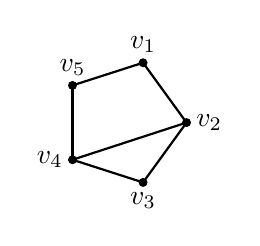
\begin{tikzpicture}[scale=0.8]
                \coordinate (b) at (0.31,0.95);
                \coordinate (c) at (1,0);
                \coordinate (d) at (0.31,-0.95);
                \coordinate (e) at (-0.81,-0.59);
                \coordinate (f) at (-0.81,0.59);
    
                \draw[fill] (b) circle (1.75pt);
                \draw[fill] (c) circle (1.75pt);
                \draw[fill] (d) circle (1.75pt);
                \draw[fill] (e) circle (1.75pt);
                \draw[fill] (f) circle (1.75pt);
    
                \draw[thick] (b)--(c);
                \draw[thick] (c)--(d);
                \draw[thick] (d)--(e);
                \draw[thick] (e)--(f);
                \draw[thick] (b)--(f);
                \draw[thick] (c)--(e);
                
                \node[above] at (0.31,0.95) {\(v_1\)};
                \node[right] at (1,0) {\(v_2\)};
                \node[below] at (0.31,-0.95) {\(v_3\)};
                \node[left] at (-0.81,-0.59) {\(v_4\)};
                \node[above] at (-0.81,0.59) {\(v_5\)};
    \end{tikzpicture}
    \end{equation}

    Where the edges are oriented with the larger vertex index at the head and smaller at the tail. Compute generators for the cycles, and show that \(C_*(G) \simeq C_*(G')\) as chain complexes, where \(G'\) is \(G\) with \((v_1,v_5)\) replaced with \((v_5,v_1)\). Finally, show that \(H_1(G) \cong H_1(G')\)
    
    \emph{proof - }
    We can write \(d_1\) as a matrix,
    \begin{align*}
        \begin{bmatrix} -1 & 0 &0 &0 &0 &-1 \\ 1 &-1 &-1 &0 &0 &0  \\ 0 & 1& 0&-1&0 &0  \\ 0 &0 &1 &1 &-1 &0 \\ 0 & 0&0 &0 & 1& 1 \end{bmatrix} \overset{\text{Row Reduction}}{\rightsquigarrow} \begin{bmatrix} -1&0&0&0&0&-1\\0&-1&-1&0&0&-1\\0&0&-1&-1&0&-1\\0&0&0&0&-1&-1\\0&0&0&0&0&0\end{bmatrix}
    \end{align*}
    So the kernel has rank 2.
    From this matrix we can compute generators for the kernel, (and thus the cycles)
    \[\ker d_1 = (e_2-e_4,e_1+e_5-e_6)\]

    To show that \(C_*(G)\), and \(C_*(G')\) are chain homotopic, define \[f:v_i \mapsto v_i', e_i \mapsto e_i', \quad g: v_i' \mapsto v_i, e_i' \mapsto e_i\].
    By construction these are chain maps, since firstly \(d_0 = 0, d_0' = 0\), and \(e_i = e_i'\) for each \(e_i \neq (v_1,v_5)\), and the values of \(d_1\) agree with \(d_1'\) on each of the equal \(e_i = e_i'\). For \(e = (v_1,v_5), e' = (v_5,v_1)\), we have \(f_1(e) = -e',g_1(e')=-e\), for \(e \neq (v_1,v_5), e' \neq (v_5,v_1)\) commutativity is obvious since \(d(e) = d'(e')\) in this case. For \(e = (v_1,v_5)\) we have \(f_0 \circ d(e) = f_0(x-y) = x-y = -(y-x) = -d_1'(e') = d_1'(f_1(e))\), the argument is the exact same for commutativity of the square replacing \(g\) for \(f\) and \(e'\) for \(e\). Then \(f \circ g = 1\), so we can just choose our homotopy to be the zero map.

    To see that the homology is the same, there are 2 possible solutions both are easy. The first is that they are isomorphic as chain complexes, the second is that \(d_1\) is rewritten by multiplying a row by \(-1\), preserving the row reduced form and hence the generators of the kernel. \qed



    %%%%%%%%%%%%%%%%%%%%%%%%%%%%%%%%%%%%%%%%%%%%%%%%%%%%%%%%%%%%%%%%%%%%%%%%%%%%%%%%%%%%%%%%%%%%%%%%%%%%%%%%%%%%%%%%%%%%%%%%%%%%%%%%%%%%%%%

    
    \emph{exercise - }\label{HEx4} Let \(\Gamma, \Gamma'\) be arbitrary graphs such that \(\Gamma \simeq \Gamma'\), then \(C_*(\Gamma) \simeq C_*(\Gamma')\)

    \emph{proof - } In (i) we show that homotopy of graphs is independent of orientation, and in (ii), we show that it is equivalent up to quotienting by an edge between to vertices, this is sufficient since it allows us to show that (since the graphs are homotopic they have the same Euler characteristic)
    \[C_*(\Gamma) \simeq C_*(\bigvee_{1 \leq k \leq \chi(\Gamma)} S^1) \simeq C_*(\Gamma')\]

    (i) Assume that \(\Gamma\setminus e_0 = \Gamma' \setminus e_0'\), such that \(e_0' = -e_0\), we copy the proof in the previous question.
    \begin{align*}
        f: &C_*(\Gamma) \to C_*(\Gamma')
        &\begin{cases}
            e_0 \mapsto -e_0' \\
            e_i \mapsto e_i' & i \geq 1 \\
            v_i \mapsto v_i'
        \end{cases}
        g: &C_*(\Gamma') \to C_*(\Gamma)
        &\begin{cases}
            e_0' \mapsto -e_0 \\
            e_i' \mapsto e_i & i \geq 1 \\
            v_i' \mapsto v_i
        \end{cases}
    \end{align*}
    \(fg = 1_{C_*(\Gamma)}\), \(gf = 1_{C_*(\Gamma')}\), so they are homotopies so long as they are chain maps. This is trivial except for the "square" where edges map to vertices.
    Commutativity on generators is trivial apart from \(e_0\), and \(e_0'\), in this case \(f\circ d_1(e_0) = f(v_1 - v_0) = v_1' - v_0' = -(v_0' - v_1') = d_1'(-e_0') = d_1'\circ f (e_0)\). The proof is the same for \(g\).

    (ii) Suppose we are quotienting the edge \(e_0 = (v_0,v_1), v_0 \neq v_1\). Here in order to focus on the most relevant parts of the chain complex we do some book keeping:
    \begin{align*}
        &C_*(\Gamma)_2 = \mathbb{Z}_0^2 \oplus S_2 &C_*(\Gamma)_1 = \mathbb{Z}_0^1 \oplus \mathbb{Z}_1^1 \oplus S_1 \\
        &C_*(\Gamma')_2 = S_2' &C_*(\Gamma')_1 = \mathbb{Z}_0' \oplus S_1'
    \end{align*}
    Here there are natural identifications of all edges and vertices in \(S_i \tand S_i'\). There is really only one way to define \(f\) if we want to keep the natural mapping \(f: S_i \to S_i'\),
    \begin{align*}
        &f_1: (a_0e_0,a_1e_1,\hdots,a_me_m) \mapsto (a_1\overline{e_1},a_2\overline{e_2},\hdots,a_m\overline{e_m}) \\
        &f_0:(a_0v_0,a_1v_1,\hdots,a_nv_n) \mapsto ((a_0+a_1)\overline{v_1},a_2\overline{v_2},\hdots,a_n\overline{v_n})
    \end{align*}
    It is clear that \(f\) is a chain map from construction. Now we define \(g: C_*(\Gamma') \to C_*(\Gamma)\) as follows,
    \begin{align*}
        g_0: (a_1\overline{v_1},\hdots,a_n\overline{v_n}) \mapsto (0,a_1v_1,\hdots,a_nv_n)
    \end{align*}
    Then taking the natural map \(S_2' \to S_2\), composition with \(d\) gives \(e_i \mapsto \sum_{j=0}^nk_j^iv_j\), define \(g_1: \overline{e_i} \mapsto k^i_0e_0 + e_i\). Then we have \(\overline{k_1^i} = k_0^i + k_1^i\)
    \[d_1g_1(\overline{e_i}) = d_1(k_0^ie_0 + e_i) = k_0^i(v_1 - v_0) + \sum_{j=0}^n k_j^i v_j\]
    \[g_0\overline{d_1}(\overline{e_i}) = g_0\left(\sum_{j=1}^n \overline{k_j^i} \overline{v_j}\right) = g_0\left((k_0^i + k_1^i)\overline{v_1} + \sum_{j=2}^n k_j^i \overline{v_j}\right) = \sum_{j=0}^n k_j^i v_j + k_0^i(v_1 - v_0)\]
    This implies that \(g\) is indeed a chain map. It is immediate that \(fg = 1_{C_*(\Gamma')}\), we need to provide a homotopy to show that \(gf \simeq 1_{C_*(\Gamma)}\). Explicitly we have
    \begin{align*}
        &1 - g_1f_1 = \left(a_0 - \sum_1^m a_i k_0^i\right)e_0 \\
        &1 - g_0f_0 = a_0(v_0 - v_1)
    \end{align*}
    the map \(h: v_0 \mapsto -e_0\) obviously satisfies \(d_1h_1(a_0,\hdots,a_n) = a_0(v_0 - v_1)\). We only need to check that \(h_1d_1 = \left(a_0 - \sum_1^m a_i k_0^i\right)e_0\), but the first coordinate of \(d_1(a_0e_0 + \sum_{i=1}^m a_i e_i)\) is \(-a_0 + \sum_{i=1}^m a_ik_0^i\), by definition of \(k_0^i\), and since \(e_0 = (v_0,v_1)\). It follows that \[h_1\circ d_1(a_0e_0 + \sum_{i=1}^m a_i e_i) = -(-a_0 + \sum_{i=1}^m a_ik_0^i)e_0 = 1-g_1f_1 \qed\]

    %%%%%%%%%%%%%%%%%%%%%%%%%%%%%%%%%%%%%%%%%%%%%%%%%%%%%%%%%%%%%%%%%%%%%%%%%%%%%%%%%%%%%%%%%%%%%%%%%%%%%%%%%%%%%%%%%%%%%%%%%%%%%%%%%%%%%%%


    \emph{exercise - }\label{HEx5} Using the cell structures for \(S^2\) from \(e^2 \cup e^0\), \(e^2 \cup e^2 \cup e^1 \cup e^0\) Build \(C_*(S^2)\) and compute its Homology.

    \emph{proof - } The first cell structure gives the sequence

    \begin{equation*}
        \begin{tikzcd}
            0 \arrow[r] & \mathbb{Z} \arrow[r] & 0 \arrow[r] & \mathbb{Z} \arrow[r] & 0
        \end{tikzcd}
    \end{equation*}

    In this case the homology modules are trivially \(H_i(C_*(S^2)) = \begin{cases}
        0 & i \neq 0,2 \\
        1 & i = 0,2
    \end{cases}\)

    The second cell structure gives the sequence

    \begin{equation*}
        \begin{tikzcd}
            0 \arrow[r] & \mathbb{Z}e_0^2 \oplus \mathbb{Z}e_1^2 \arrow[r,"{d_2}"] & \mathbb{Z}e_0^1 \arrow[r,"{d_1}"] & \mathbb{Z}e_0^0 \arrow[r] & 0
        \end{tikzcd}
    \end{equation*}

    Where \(\mathbb{Z}e_0^2 \oplus \mathbb{Z}e_1^2 = \mathbb{Z}\gen{e_0^2 + e_1^2} \oplus \mathbb{Z}\gen{e_0^2 - e_1^2}\), and \(d_2: e_0^2 \mapsto e_0^1, e_1^2 \mapsto -e_0^1\), so that
    \begin{align*}
        H_2(C_*(S^2)) = \frac{\mathbb{Z}\gen{e_0^2 + e_1^2} \oplus \mathbb{Z}\gen{e_0^2 - e_1^2}}{\mathbb{Z}\gen{e_0^2 + e_1^2}} \cong \mathbb{Z}
    \end{align*}
    And \(d_1: e_0^1 \mapsto e_0^0 - e_0^0\), so that \(d_1 \equiv 0\) which gives us \(H_0(C_*(S^2)) = \mathbb{Z}\), and \(H_1(C_*(S^2)) = \mathbb{Z}/\mathbb{Z} \cong 0\), with \(H_i = 0\) for \(i > 2\). The same result as above.
    



    %%%%%%%%%%%%%%%%%%%%%%%%%%%%%%%%%%%%%%%%%%%%%%%%%%%%%%%%%%%%%%%%%%%%%%%%%%%%%%%%%%%%%%%%%%%%%%%%%%%%%%%%%%%%%%%%%%%%%%%%%%%%%%%%%%%%%%%

    \emph{exercise - }\label{HEx6} Show that "augmentation" still gives a chain complex, i.e. \(\epsilon\circ d_1 = 0\) \textcolor{red}{cite Augmentation in notes}

    \emph{proof - } It will suffice to check on generators of \(C_1\), let \(e^1_\beta \in C_1\), then 
    \[\epsilon d_1(e^1_\beta) = \epsilon (e_\alpha^0 - e_{\alpha'}^0) = 1-1 = 0\]

    %%%%%%%%%%%%%%%%%%%%%%%%%%%%%%%%%%%%%%%%%%%%%%%%%%%%%%%%%%%%%%%%%%%%%%%%%%%%%%%%%%%%%%%%%%%%%%%%%%%%%%%%%%%%%%%%%%%%%%%%%%%%%%%%%%%%%%%

    \emph{exercise - }\label{HEx7} \(S^1 \wedge S^1 \simeq S^2\)

    \emph{proof - } \(S^1 \wedge S^1 \cong \frac{T^2}{S^1 \vee S^1}\), where \(T^2 \cong D^2/\sim\), then
    \begin{align*}
        S^1 \wedge S^1 = \frac{T^2}{S^1 \vee S^1} \cong \frac{D^2/\sim}{\partial D^2} = \frac{D^2}{\partial D^2} \cong S^2
    \end{align*}

    %%%%%%%%%%%%%%%%%%%%%%%%%%%%%%%%%%%%%%%%%%%%%%%%%%%%%%%%%%%%%%%%%%%%%%%%%%%%%%%%%%%%%%%%%%%%%%%%%%%%%%%%%%%%%%%%%%%%%%%%%%%%%%%%%%%%%%%

    \emph{exercise - }\label{HEx8} \(SX \simeq \sum X\)

    \emph{proof - } Here \((X,\set{*})\) is a (pointed but ignore the point for now) CW-complex, we can give \(X \times I\) a CW structure, note that we have \(\partial e^n = \partial(e^{n-1} \times I) = (\partial e^{n-1} \times I)\cup e^{n-1} \times \partial I\)
    (we can do this using point set topology and the fact that the sets are closed), then the CW-structure on \((X \times I)^n\) can be taken to be \((X \times I)^0 = X^0 \times \partial I\), then taking \(\varphi_\alpha^n\) to be the gluing map of \(e_\alpha^{n}\) into \(X^n\):
    \begin{align*}
        (X \times I)^n = (X \times I)^{n-1} \bigcup_{\varphi_\alpha^n} e_\alpha^n \times \partial I \bigcup_{\varphi_\alpha^{n-1} \times I} e_\alpha^{n-1} \times I
    \end{align*}
    This gives a CW structure on \(X \times I\) with \(X \times \partial I\) as a substructure, there is a canonical CW structure on the quotient given by replacing \(\varphi_\alpha^n\) with \(\pi\vert_{X^n} \circ\varphi_\alpha^n\). Furthermore since \(* \in X^0\), we have \(\set{*} \times I \in (X \times I)^1\), which can be identified with its image in the quotient. This is a contractible subcomplex, so by the CW extension theorem
    \begin{align*}
        SX = \frac{X \times I}{X \times \partial I} \cong \frac{X \times I}{X \times \partial I \cup \set{*} \times I} = \sum X
    \end{align*}
    
    %%%%%%%%%%%%%%%%%%%%%%%%%%%%%%%%%%%%%%%%%%%%%%%%%%%%%%%%%%%%%%%%%%%%%%%%%%%%%%%%%%%%%%%%%%%%%%%%%%%%%%%%%%%%%%%%%%%%%%%%%%%%%%%%%%%%%%%

    \emph{exercise - }\label{HEx9} \(X \wedge S^1 \simeq \sum X\)

    \emph{proof - } It is important here that the same point \(x \in X\) is used in either quotient. Consider the map \(f: I \to S^1, t \mapsto e^{i\pi t}\), then we get the following,
    \begin{equation*}
        \begin{tikzcd}
            X \times I \arrow[d,"{\pi}"] \arrow[r,"{1 \times f}"] & X \times S^1 \arrow[d,"{\pi'}"] \\
            \frac{X \times I}{X \times \set{1} \cup X \times \set{-1} \cup \set{x}\times I} \arrow[r,"{\overline{1 \times f}}"] &\frac{X \times S^1}{X\times \set{1} \cup \set{x} \times S^1}
        \end{tikzcd}
    \end{equation*}

    The bottom left here is the (reduced) suspension \(\sum X\), and the bottom right is \(X \wedge S^1\). Here the induced map is clearly bijective, since the quotients here are equivalent to quotienting by the image of the quotients, along with quotienting on the left side \(f^{-1}(1) \times \set{1} \sim f^{-1}(-1) \times \set{-1} \sim x\), where \(f\) wasn't injective. Continuity of the inverse follows, since we have \(\frac{X \times I}{X \times \partial I} \cong X \times S^1\), and we can factor our map through this homeomorphism before taking quotients.
    %%%%%%%%%%%%%%%%%%%%%%%%%%%%%%%%%%%%%%%%%%%%%%%%%%%%%%%%%%%%%%%%%%%%%%%%%%%%%%%%%%%%%%%%%%%%%%%%%%%%%%%%%%%%%%%%%%%%%%%%%%%%%%%%%%%%%%%

    \emph{exercise - }\label{HEx10} Use \(\tilde{H_i}\) to show that \(\partial D^n\) cannot be a retract of \(D^n\)

    \emph{proof - } We have that \(D^n/\partial D^n \cong S^n\), furthermore \(D^n \simeq \set{x}\) for all \(n\), implying that \(\tilde{H}_i(D^n) \cong \tilde{H}_i(\set{x}) = 0\), for any \(i,n \in \mathbb{Z}_{\geq 0}\). Suppose for contradiction that there were a retract \(h: D^n \to \partial D^n\), then denoting \(\iota: \partial D^n \hookrightarrow D^n\) we would have that \(h \circ \iota \simeq 1_{\partial D^n}\), by functoriality we get the following commutative diagram (also note that \(\partial D^n = S^{n-1}\)):

    \begin{equation*}
        \begin{tikzcd}
            \tilde{H}_{n-1}(\partial D^n) \arrow[r,"{1}"] \arrow[d,"{\iota_*}"] &\tilde{H}_{n-1}(\partial D^n) \\
            \tilde{H}_{n-1}(D^n) \arrow[ur,"{h_*}"]
        \end{tikzcd}
    \end{equation*}
    Where this diagram is equivalent to
    \begin{equation*}
        \begin{tikzcd}
            \mathbb{Z} \arrow[r,"{1}"] \arrow[d] &\mathbb{Z} \\
            0 \arrow[ur]
        \end{tikzcd}
    \end{equation*}
    This is clearly a contradiction since there are no surjective morphisms \(0 \to \mathbb{Z}\). \qed

    % \begin{equation*}
    %     \begin{tikzcd}
    %         \tilde{H}_n(\partial D^n) \arrow[r] & \tilde{H}_n(D^n) \arrow[r] & \tilde{H}_n(D^n/\partial D^n) \arrow[r] & \tilde{H}_{n-1}(\partial D^n) \arrow[r] & \tilde{H}_{n-1}(D^n) \arrow[r] & \tilde{H}_{n-1}(D^n/\partial D^n) \\
    %         \tilde{H_n}(S^{n-1}) \arrow[r] & \tilde{H_n}(D^n) \arrow[r] & \tilde{H_n}(S^n) \arrow[r] & \tilde{H}_{n-1}(S^{n-1}) \arrow[r] &\tilde{H}_{n-1}(D^n) \arrow[r] & \tilde{H}_{n-1}(S^n)\\
    %         0 \arrow[r] & \tilde{H_n}(D^n) \arrow[r] & \mathbb{Z} \arrow[r] & \mathbb{Z} \arrow[r] &\tilde{H_{n-1}}(D^n) \arrow[r] & 0
    %     \end{tikzcd}
    % \end{equation*}

    %%%%%%%%%%%%%%%%%%%%%%%%%%%%%%%%%%%%%%%%%%%%%%%%%%%%%%%%%%%%%%%%%%%%%%%%%%%%%%%%%%%%%%%%%%%%%%%%%%%%%%%%%%%%%%%%%%%%%%%%%%%%%%%%%%%%%%%

    \emph{exercise - }\label{HEx11} Let \(f: S^n \to S^n\), show if \(f\) is not surjective then \(\deg f = 0\)

    \emph{proof - } Suppose that \(f\) is not surjective, then we can pick some \(x \in S^n \setminus f(S^n)\), by the stereographic projection \(S^n \setminus \set{x} \cong \mathbb{R}^n \simeq \set{*}\), so we have the following commutative diagram, where the downward map is taken by restricting the codomain of \(f\) to \(S^n \setminus \set{x}\), and the upper diagonal is the inclusion.
    \begin{equation*}
        \begin{tikzcd}
            \tilde{H_n}(S^n) \arrow[r,"{f_*}"] \arrow[d] &\tilde{H_n}(S^n) \\
            \tilde{H_n}(\set{*}) \arrow[ur]
        \end{tikzcd}
    \end{equation*}
    equivalently,
    \begin{equation*}
        \begin{tikzcd}
            \mathbb{Z} \arrow[r,"{f_*}"] \arrow[d] &\mathbb{Z} \\
            0 \arrow[ur]
        \end{tikzcd}
    \end{equation*}
    so \(f_*\) must be the zero map.

    %%%%%%%%%%%%%%%%%%%%%%%%%%%%%%%%%%%%%%%%%%%%%%%%%%%%%%%%%%%%%%%%%%%%%%%%%%%%%%%%%%%%%%%%%%%%%%%%%%%%%%%%%%%%%%%%%%%%%%%%%%%%%%%%%%%%%%%

    \emph{exercise - }\label{HEx12} Let \(f\) as in the previous exercise, show that \(\deg f = \deg \sum_* f \) (remark first  show that the suspension \(\sum\) is functorial)

    \emph{proof - } given \(f: X \to Y\), we can define \(\sum_* f\) as the induced map in the following diagram
    \begin{equation*}
        \begin{tikzcd}
            X \times I \arrow[d,"{\pi_X}"] \arrow[r,"{f \times 1}"]& Y \times I \arrow[d,"\pi_Y"] \\
            \sum X \arrow[r,"{\sum_* f}"]& \sum Y
        \end{tikzcd}
    \end{equation*}
    Continuity simply follows from continuity of \(f\), and the definition of quotient topology taking opens to opens on the upper half of the square, then commutativity and the universal property of the quotient on the lower square. To get \(\sum_* fg = \sum_*f \sum_*g\) simply factor \(f\circ g \times 1\) through the following diagram
    \begin{equation*}
        \begin{tikzcd}
            X \times I \arrow[d,"{\pi_X}"] \arrow[r,"{f \times 1}"]& Y \times I \arrow[d,"\pi_Y"] \arrow[r,"{g \times 1}"] &Z \times I \arrow[d,"{\pi_Z}"] \\
            \sum X \arrow[r,"{\sum_* f}"]& \sum Y \arrow[r,"{\sum_* g}"]& \sum Z
        \end{tikzcd}
    \end{equation*}
    \(\sum_*1 = 1_{\sum_*}\) is obvious. This suffices to show functoriality.

    For the proof of the main result, note that by an identical construction, the canonical \(C_*\) is functorial, \(f: X \to Y\), then \(C_*f : C_{1_X} \to C_{1_Y}\). It suffices to show the following result for \(SX\), since it has the same Homology as \(\sum X\) by homotopy equivalence, so factoring \(f\) through this equivalence won't affect the degree. We have naturality (identifying \(S^n \leftrightarrow S^n \times \set{0} f \leftrightarrow C_*f \vert_{S^n \times \set{0}}\))
    \begin{equation*}
        \begin{tikzcd}
            S^n \arrow[d,"{f}"] \arrow[r]& CS^n\arrow[d,"{C_*f}"]\\
            S^n \arrow[r]& CS^n 
        \end{tikzcd}
    \end{equation*}
    And hence, we get a chain map
    \begin{equation*}
        \begin{tikzcd}
            H_{n+1}(CS^n) \arrow[d,"{(C_*f)_*}"] \arrow[r,"{}"]& H_{n+1}(CS^n,S^n) \arrow[d,"{(S_*f)_*}"]\arrow[r,"{}"]& H_n(S^n)\arrow[d,"{f_*}"] \arrow[r,"{}"]& H_n(CS^n) \arrow[d,"{(C_*f)_*}"] \\
            H_{n+1}(CS^n)\arrow[r,"{}"]& H_{n+1}(CS^n,S^n) \arrow[r,"{}"]& H_n(S^n) \arrow[r,"{}"]& H_n(CS^n)
        \end{tikzcd}
    \end{equation*}
    Which we can rewrite as
    \begin{equation*}
        \begin{tikzcd}
            0 \arrow[d,"{(C_*f)_*}"] \arrow[r,"{}"]& H_{n+1}(S(S^n)) \arrow[d,"{(S_*f)_*}"]\arrow[r,"{}"]& H_n(S^n)\arrow[d,"{f_*}"] \arrow[r,"{}"]& 0 \arrow[d,"{(C_*f)_*}"] \\
            0\arrow[r,"{}"]& H_{n+1}(S(S^n)) \arrow[r,"{}"]& H_n(S^n) \arrow[r,"{}"]& 0
        \end{tikzcd}
    \end{equation*}
    Commutativity suffices to show that the degrees of the maps must be equal. \qed
    
    \textbf{Remark 1.} Use of the \(0\) maps on either end of the sequence is a bit of a cheat here so we get for free that \(H_{n+1}(S(S^n)) \cong \mathbb{Z}\), and we need to ensure the map \(H_{n+1}(S(S^n)) \to H_n(S^n)\) is nonzero since otherwise we cannot conclude about \((\sum_*f)_*(1) = (S_*f)_*(1)\) from the above diagram.

    \textbf{Remark 2.} To make sense of degree here we should really show that \(\sum S^n \simeq S(S^n) \simeq S^{n+1}\), there is an explicit homeomorphism by simply rescaling by the factor in \(I\) in \(S^n \times I\), then taking the quotient.


    %%%%%%%%%%%%%%%%%%%%%%%%%%%%%%%%%%%%%%%%%%%%%%%%%%%%%%%%%%%%%%%%%%%%%%%%%%%%%%%%%%%%%%%%%%%%%%%%%%%%%%%%%%%%%%%%%%%%%%%%%%%%%%%%%%%%%%%

    \emph{exercise - }\label{HEx13} Compute the Homology of \(X\), where \(X\) is the triangulation of the Torus.

    \emph{proof - } Let the upper triangle be \(e_U^2\), the lower triangle be \(e_L^2\), the upper/lower boundary be \(e_\alpha^1\), the left/right boundary be \(e_\beta^1\), and the diagonal be \(e_\gamma^1\), there is only one zero-cell, we may call it \(e^0\). Then:
    \begin{align*}
        \pi_\alpha \varphi_U = \pi_\beta \varphi_U = 1 = - \pi_\gamma \varphi_U \\
        \pi_\alpha \varphi_L = \pi_\beta \varphi_L = -1 = - \pi_\gamma \varphi_L \\
        \pi_0 \varphi_\alpha = \pi_0 \varphi_\beta = \pi_0 \varphi_\gamma = 1 - 1 = 0
    \end{align*}

    In this case we have the cell structure
    \begin{equation*}
        \begin{tikzcd}
            0 \arrow[r] & \mathbb{Z}\gen{e^2_U} \oplus \mathbb{Z}\gen{e^2_L} \arrow[r,"{d_2}"] & \mathbb{Z} \gen{e^1_\alpha} \oplus \mathbb{Z} \gen{e^1_\beta} \oplus \mathbb{Z} \gen{e^1_\gamma} \arrow[r,"{d_1}"] &\mathbb{Z} \gen{e^0} \arrow[r] & 0
        \end{tikzcd}
    \end{equation*}
    Where \(\ker d_2 = e_U^2 + e_L^2\), \(d_1 = 0 = d_0\), rewriting \(C_1(X)\) to have \(\text{Im}\,C_2(X)\) as one of its three generators, we get the usual Homology modules for the Torus
    \begin{align*}
        H_2(X) \cong \mathbb{Z}, \quad H_1(X) \cong \mathbb{Z} \oplus \mathbb{Z}, \quad H_0(X) \cong \mathbb{Z}
    \end{align*}


    %%%%%%%%%%%%%%%%%%%%%%%%%%%%%%%%%%%%%%%%%%%%%%%%%%%%%%%%%%%%%%%%%%%%%%%%%%%%%%%%%%%%%%%%%%%%%%%%%%%%%%%%%%%%%%%%%%%%%%%%%%%%%%%%%%%%%%%

    \emph{exercise - }\label{HEx14} Show from the Homology axioms that \(\tilde{H_n}(X^{n+1}) = \tilde{H_n}(X)\)

    \emph{proof - } We have from Axiom 1, the following sequence is exact
    \begin{equation*}
        \begin{tikzcd}
            \tilde{H}_{k+1}(X^{m+1}/X^m) \arrow[r] & \tilde{H}_{k}(X^m) \arrow[r] & \tilde{H}_{k}(X^{m+1}) \arrow[r] & \tilde{H}_{k}(X^{m+1}/X^m)
        \end{tikzcd}
    \end{equation*}
    We have the following from construction of a CW complex:
    \begin{align*}
        X^{n+1}/X^n = \frac{\frac{e_\alpha^{n+1} \bigsqcup_\alpha X^n}{x \sim \varphi_\alpha(x),\; x \in \partial e_\alpha^{n+1},\; \varphi_\alpha(x) \in X^n}}{X^n} = \frac{\bigsqcup_\alpha e_\alpha^{n+1}}{\bigsqcup_{\alpha}\partial e_\alpha^{n+1}} \cong \bigvee_\alpha S^{n+1}
    \end{align*}
    So for \(k \neq m+1,m\) we have
    \begin{equation*}
        \begin{tikzcd}
            0 \arrow[r] & \tilde{H}_{k}(X^m) \arrow[r] & \tilde{H}_{k}(X^{m+1}) \arrow[r] & 0
        \end{tikzcd}
    \end{equation*}
    by exactness this gives an isomorphism \(\tilde{H}_n(X^{n+1}) \cong \tilde{H}_n(X^{n+2}) \cong \cdots \cong \tilde{H}_n(X)\)
    

    %%%%%%%%%%%%%%%%%%%%%%%%%%%%%%%%%%%%%%%%%%%%%%%%%%%%%%%%%%%%%%%%%%%%%%%%%%%%%%%%%%%%%%%%%%%%%%%%%%%%%%%%%%%%%%%%%%%%%%%%%%%%%%%%%%%%%%%

    \emph{exercise - }\label{HEx15} Rewrite Homoology axioms (1-3) in the context of the category \textbf{Pairs}

    \emph{proof - } First note that functoriality gives homotopy invarience, homotopy equivalent maps \(f,g:(X,A) \to (Y,B), \; f \simeq g\) (here we mean the restrictions induce homotopy equivalences on the smaller spaces) induce the same maps of homology modules \(f_* = g_*: H_n(X,A) \to H_n(X,B)\)
    \begin{enumerate}
        \item The following sequence is long exact:
        \begin{equation*}
            \begin{tikzcd}
                \cdots H_{n+1}(X,A) \arrow[r] & H_n(A,\set{*}) \arrow[r] & H_n(X,\set{*}) \arrow[r] &H_n(X,A) \arrow[r] &\cdots
            \end{tikzcd}
        \end{equation*}
        \item For any \(n\), \(H_n\left(\bigvee_\alpha (X_\alpha,A_\alpha)\right) = \bigoplus_\alpha H_n(X_\alpha,A_\alpha)\), here we are quotienting an element in \(A, B\) resp. when we take \((X,A)\vee(Y,B)\)
        \item \(H_n(S^0,\set{*}) = \begin{cases}
            \mathbb{Z} & n=0 \\ 0 & n > 0
        \end{cases}\)
    \end{enumerate}

    %%%%%%%%%%%%%%%%%%%%%%%%%%%%%%%%%%%%%%%%%%%%%%%%%%%%%%%%%%%%%%%%%%%%%%%%%%%%%%%%%%%%%%%%%%%%%%%%%%%%%%%%%%%%%%%%%%%%%%%%%%%%%%%%%%%%%%%

    \emph{exercise - }\label{HEx16} Let \(X\) be a cell complex with subcomplex \(A\), furthermore let \(K \subset A\) be any set such that \(\overline{K} \subset A^\circ\), show that
    \begin{align*}
        \frac{X \setminus K}{A \setminus K} \simeq X/A
    \end{align*}

    \emph{proof - } We get the following commutative diagram, since \(\iota: X \setminus K \hookrightarrow X\) is such that \(\iota \vert_{A \setminus K} : A \setminus K \hookrightarrow A\)

    \begin{equation*}
        \begin{tikzcd}
            X \setminus K \arrow[r,"{\iota}"] \arrow[d,"{\pi_1}"] & X \arrow[d,"{\pi_2}"] \\
            \frac{X \setminus K}{A \setminus K} \arrow[r,"{\overline{\iota}}"] & X/A
        \end{tikzcd}
    \end{equation*}

    The induced map is clearly bijective, since \(\iota\) is bijective on \(A^c\). Continuity of \(\overline{\iota}\) follows from continuity of \(\iota\). To see that \(\overline{\iota}^{-1}\) is continuous, let \(U\) be open  in \(X\), if \(\set{a} \not \in U\) (here \(\set{a} \subset A \setminus K\)), then \(\pi_1^{-1}(U) = \pi_1^{-1}(U) \cap \overline{K}^c\), so \(\iota(\pi_1^{-1}(U) \cap \overline{K}^c) = \pi_2^{-1}(\overline{\iota}(U))\) which the former is open in the subspace topology iff it is open in \(X\). Now if \(\set{a} \subset U\), then \(\pi_2^{-1}\overline{\iota}(U) = \iota\pi_1^{-1}(U) \cup A^\circ\), where \(\iota\pi_1^{-1}(U) = V \cap K^c\), where \(V\) is open in \(X\), rewriting this we get \(\pi_2^{-1}\overline{\iota}(U) = V \cup A^\circ\) which is open in \(X\), so \(\overline{\iota}(U)\) is open in the quotient topology. \qed


    %%%%%%%%%%%%%%%%%%%%%%%%%%%%%%%%%%%%%%%%%%%%%%%%%%%%%%%%%%%%%%%%%%%%%%%%%%%%%%%%%%%%%%%%%%%%%%%%%%%%%%%%%%%%%%%%%%%%%%%%%%%%%%%%%%%%%%%

    \emph{exercise - }\label{HEx17} Compute \(\tilde{H_i}(\mathbb{RP}^n)\)

    \emph{proof - } We compute this using cellular homology and degree. First a lemma,

    \textbf{Lemma.} The antipodal map \(f: S^n \to S^n, x \mapsto -x\) is such that \(\deg f = (-1)^{n+1}\)

    Proof of lemma: Consider the CW structure \(e_U^n \cup e_L^n \cup e^{n-1} \cup e^0\) on \(S^n\), \(\tilde{H}_k(S^n) = 0\) unless \(k=n\), so we just consider \(k=n\). It follows that the map \(r: e_U^n \leftrightarrow e_L^n\) on \(\tilde{H}_n(S^n) = \mathbb{Z}\gen{e_U^n - e_L^n}\) takes \(1 \mapsto -1\), so \(r\) has degree \(-1\). Now taking one \(r_i\) for each coordinate plane in \(\mathbb{R}^{n+1}\), we have \(f = \prod_{i=1}^{n+1} r_i \simeq r^{n+1}\) (rotations are homotopies), hence \(\deg f = \deg r^{n+1} = (\deg r)^{n+1} = (-1)^{n+1}\). \qed

    Continuing with the proof of the theorem, we give \(\mathbb{RP}^n\) the usual cell structure, i.e. since
    \begin{align*}
        &\mathbb{RP}^n \cong S^n/\!\!\sim \;\cong \frac{D^n}{\sim_{\partial D^n}} = \frac{D^n}{\sim_{S^{n-1}}}
    \end{align*}
    we find that taking \(\varphi_n\) as the identity map \(\partial D^n \to S^{n-1}\)
    \begin{align*}
        \mathbb{RP}^n = e^n \cup_{\varphi_n} \mathbb{RP}^{n-1} = e^n \cup_{\varphi_n} e^{n-1} \cup_{\varphi_{n-1}} \cdots \cup_{\varphi_0} e^0
    \end{align*}
    This gives a chain complex:
    \begin{equation*}
        \begin{tikzcd}
            C_{n+1}(\mathbb{RP}^n) \arrow[r] &C_n(\mathbb{RP}^n) \arrow[r] &C_{n-1}(\mathbb{RP}^n) \arrow[r] &C_{n-2}(\mathbb{RP}^n) \arrow[r] &\cdots \arrow[r] &C_0(\mathbb{RP}^n) \arrow[r] & 0 \\
            0 \arrow[r] &\mathbb{Z} \arrow[r] &\mathbb{Z} \arrow[r] &\mathbb{Z} \arrow[r] &\cdots \arrow[r] &\mathbb{Z} \arrow[r] & 0
        \end{tikzcd}
    \end{equation*}
    We want to use degree to compute \(d_k\). In this case, we only have one \(n-1\)-cell and we are attaching only one \(n\)-cell, so the we can determine \(d_n\) from \(d_n(e^n) = (\deg f) e^{n-1}\). Where \(f\) is just the composition
    \begin{equation*}
        \begin{tikzcd}
            \partial e^n \arrow[rr,"{f}"] \arrow[rd,"{\varphi}"]&  &\frac{\mathbb{RP}^{n-1}}{\mathbb{RP}^{n-2}} \\
            &\mathbb{RP}^{n-1} \arrow[ru,"{\pi}"]
        \end{tikzcd}
    \end{equation*}
    Fix a point \(y \in \frac{\mathbb{RP}^{n-1}}{\mathbb{RP}^{n-2}}\), then \(f^{-1}(y) = \set{x,-x}\), taking neighborhoods as in the definition of local degree, we may take \(V = f(U_1)\), and \(U_2\) homeomorphic to \(V\) via \(f\) by excision on either \(U_1\) or \(U_2\). Then there is a homeomorphism \(f\vert_{U_2}f\vert_{U_1}^{-1}: U_1 \to U_2\). This map extends to the antipodal map \(r^{n+1}: \partial e^n \to \partial e^n\) which has degree \(\sigma(n+1)\), it follows that (since \(\deg g^{-1} = \deg g,\; \forall g\) invertible) we have \(\deg f \vert_{-x} = (-1)^{n+1} \deg f \vert_x\). If \(\deg f \vert_x = -1\), then this is actually arbitrary, since we could have chosen opposite generators for \(H_n(S^n)\), so we can assume that \(\deg f \vert_x = 1\). This computes \(d_n\)
    \begin{align*}
        d_n(e^n) = \deg f = \deg f \vert_x + \deg f \vert_{-x} = 1 + \sigma(n+1)
    \end{align*}
    This gives us the chain complex
    \begin{equation*}
        \begin{tikzcd}
            &\cdots \arrow[r,"{\times 2}"]& \mathbb{Z} \arrow[r,"{0}"] &\mathbb{Z} \arrow[r,"{\times 2}"] &\mathbb{Z} \arrow[r] & 0 \arrow[r]& 0
        \end{tikzcd}
    \end{equation*}
    Now we can directly compute
    \begin{align*}
        \tilde{H}_k(\mathbb{RP}^n) = \begin{cases}
            \mathbb{Z} & k=n \equiv 1\!\!\!\mod{2} \\
            \mathbb{Z}/(2) &n \geq k \equiv 1\!\!\!\mod{2}\\
            0 & \text{else}
        \end{cases}
    \end{align*}
\end{document}